%% Figure from MATH 556 notes, section 49 (Lecture 22). ADDED (not from lecture).
\begin{tikzpicture}[>=stealth, xscale=2.3, yscale=0.42]
    \draw[->] (-1.6,0) -- (2.75,0) node[right, font=\scriptsize] {$\lambda$ (real)};
    \draw[->] (-1.6,0) -- (-1.6,8.8);
    \draw[line width=2pt, blue!70!black] (0,0) -- (1,0);
    \node[blue!70!black, font=\scriptsize, below] at (0.5,-0.15) {$\sigma(M) = [0,1]$};
    \draw[thick, red!70!black, domain=-1.5:-0.125, samples=60, smooth] plot (\x, {-1/\x});
    \draw[thick, red!70!black, domain=1.125:2.6, samples=60, smooth] plot (\x, {1/(\x-1)});
    \draw[densely dotted, gray] (0,0) -- (0,8.6);
    \draw[densely dotted, gray] (1,0) -- (1,8.6);
    \node[font=\scriptsize, below] at (-1,0) {$-1$};
    \draw (-1,0) -- (-1,0.25);
    \node[font=\scriptsize, below] at (2,0) {$2$};
    \draw (2,0) -- (2,0.25);
    \node[font=\scriptsize, left] at (-1.6,1) {$1$};
    \draw (-1.6,1) -- (-1.55,1);
    \node[red!70!black, font=\scriptsize, anchor=west] at (1.45,5.2) {$\|R(\lambda; M)\| = \dfrac{1}{\operatorname{dist}(\lambda, [0,1])}$};
\end{tikzpicture}
